\documentclass[border=4pt]{standalone}
% Preámbulo común de las figuras. Cada figura es un documento standalone
% que se compila a SVG con scripts/build_figures.sh
\usepackage[utf8]{inputenc}
\usepackage{amsmath}
\usepackage{tikz}
\usepackage[american, siunitx]{circuitikz}
\usetikzlibrary{arrows.meta,calc,decorations.pathmorphing,patterns}
\tikzset{
  >={Stealth[length=2.2mm]},
  eje/.style={->, thin},
  hilo/.style={thick},
}
% Paleta común: tonos medios legibles sobre fondo claro
\definecolor{azul}{RGB}{31,94,168}
\definecolor{rojo}{RGB}{192,57,43}
\definecolor{verde}{RGB}{39,128,73}
\definecolor{naranja}{RGB}{211,120,30}
\definecolor{morado}{RGB}{125,60,152}

\begin{document}
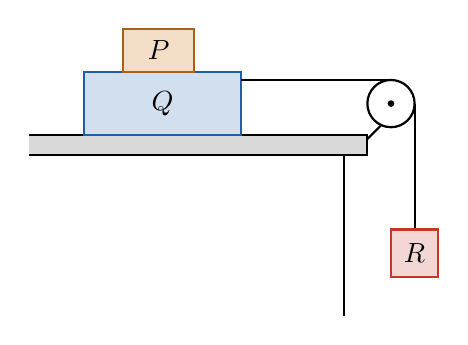
\begin{tikzpicture}[scale=1.0]
  \fill[gray!30] (-0.3,-0.25) rectangle (4.0,0);
  \draw[thick] (-0.3,0) -- (4.0,0) -- (4.0,-0.25) -- (-0.3,-0.25);
  \draw[thick] (3.7,-0.25) -- (3.7,-2.3);
  \filldraw[draw=azul, fill=azul!20, thick] (0.4,0) rectangle (2.4,0.8);
  \node at (1.4,0.4) {$Q$};
  \filldraw[draw=naranja!80!black, fill=naranja!25, thick] (0.9,0.8) rectangle (1.8,1.35);
  \node at (1.35,1.075) {$P$};
  \draw[thick] (4.0,-0.05) -- (4.3,0.25);
  \draw[thick, fill=white] (4.3,0.4) circle (0.3);
  \fill (4.3,0.4) circle (1.2pt);
  \draw[hilo] (2.4,0.7) -- (4.3,0.7);
  \draw[hilo] (4.6,0.4) -- (4.6,-1.2);
  \filldraw[draw=rojo, fill=rojo!20, thick] (4.3,-1.2) rectangle (4.9,-1.8);
  \node at (4.6,-1.5) {$R$};
\end{tikzpicture}
\end{document}
